\section{Solving quadratic equations*}

Claude likes to juggle. He throws each beanbag up in the air.  The height of a beanbag changes over time as described by the equation $$H = 3+15T-16T^2$$
where
\vspace{-.15in} %VSPACE
\begin{center}
\begin{tabular} {l} 
$H$ = height of beanbag (feet) $\sim$ dep \\
$T$ = time (seconds) $\sim$ indep \\ 
\end{tabular}
\end{center}

Let's make a table and graph this function.  For example, when $T=0$ seconds we have 
$$H = 3 + 15 \ast 0-16 \ast 0^2 = 3 + 15 \times \underline{0} - 16 \times \underline{0} \wedge 2 =  3 \text{ feet}$$
 and when $T=1$ second we have 
$$H = 3 + 15  \ast 1-16 \ast 1^2 = 3 + 15 \times \underline{1} - 16 \times \underline{1} \wedge 2 =  2 \text{ feet}$$ 

Huh?  I though the beanbag went up in the air. What's happening here?  Oh, I know.  The beanbag must be falling down by then.  
%Look at $T = .1$ seconds.  Then $$H = 3 + 15 \ast .1-16 \ast .1^2 = 3 + 15 \times \underline{.1} - 16 \times \underline{.1} \wedge 2 \approx 4.34  \text{ feet}$$  That makes more sense.  
As we fill in the table with intermediate values we see how Claude's beanbag went up in the air and then back down.

\begin{center}
\begin{tabular} {|c| |c |c |c |c |c|c |c |c|c |c  |c |c |c|}\hline
$T$ & 0 & .1 & .2 & .3 & .4 & .5 & .6 & .7 & .8 & .9 & 1 & 1.1 & 1.2 \\ \hline
$H$ & 3 & 4.34 & 5.36 & 6.06 & 6.44 & 6.50 & 6.34 & 5.66 & 4.76 & 3.54 & 2 & .14 & \cancel{$-2.04$} \\ \hline
\end{tabular}
\end{center}

Notice by $T=1.2$ seconds we got $-2.04$ feet.
%$$H = 3 + 15 \ast 1.2-16 \ast 1.2^2 = 3 + 15 \times \underline{1.2} - 16 \times \underline{1.2} \wedge 2 \approx -2.04  \text{ feet}$$  
We can't have negative feet. The beanbag must hit the ground before 1.2 seconds. From the graph I'd say in just over 1.1 seconds. 

\begin{center}
\scalebox {.8} {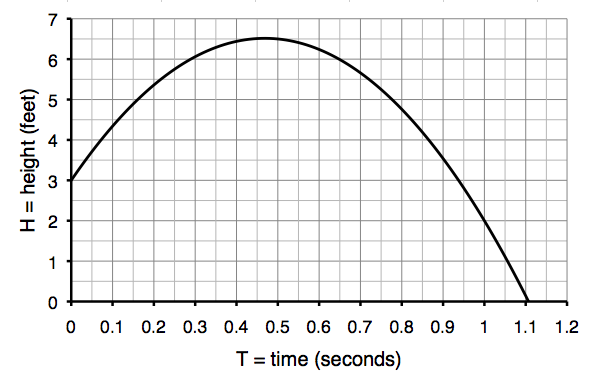
\includegraphics [width = 6in] {juggling.png}}
\end{center}

Of course, we can refine our answer by successive approximations.  The beanbag hits the ground when it's height is 0 feet.  Looks a little strange but we want $H =0$.  We expect the answer is just a little bigger than 1.1, so we start our guess optimistically with 1.11.

\begin{center}
\begin{tabular} {|c| |c  |c  |c  |c |c|}\hline
$T$ & 1.1 & 1.11 & 1.105 &1.107 & 1.106 \\ \hline
$H$ & .14& \cancel{-.06} & .0368 & \cancel{-.002} & .018 \\ \hline
vs.\ 0 & high & low & high & low  & good\\ \hline
\end{tabular}
\end{center}

\noindent The beanbag was in the air for approximately 1.106 seconds.  

In this chapter we've seen how to solve linear, power, and exponential equations.   Let's solve this equation too. By the way, our function is quadratic because $$H = 3+15T-16T^2$$ 
 fits the template for a quadratic equation that we saw earlier.  % SU 2.3 Using equations CITE?
 
\bigskip
 \framebox{
 \begin{minipage}[c]{.85\textwidth}  
~ \bigskip \\  \textsc{Quadratic equation template:} \quad $\text{dep} = a \ast \text{indep}^2 + b \ast\text{indep} + c$\\ ~ \bigskip
\end{minipage}
}
\bigskip

\noindent with constants $$a = -16 \quad b = 15 \quad c = 3$$
(More on how we found those numbers in a moment.)

Back to our juggler.  We are trying to figure out when $H=0$.  Using our equation $H=3+15T-16T^2$, we get  
$$3+15T-16T^2=0$$ 
We want  to solve for $T$. Notice that because $T$ occurs twice in the equation, nothing we have seen to do to each side of the equation can knock it down to just one $T$. That means none of our methods so far work.  Luckily there's a way to solve any quadratic equation using the aptly named \textsc{Quadratic Formula}.  

\bigskip
 \framebox{
 \begin{minipage}[c]{.85\textwidth}  
~ \bigskip \\  \textsc{Quadratic Formula:} \quad The equation $aT^2+bT+c=0$ has solutions \\ $$T = \frac{-b}{2a} \pm \frac{\sqrt{b^2-4ac}}{2a}$$ \bigskip
\end{minipage}
}
\bigskip

Oh my!  First thing to understand in this complicated formula is that we actually get two possible answers $$T = \frac{-b}{2a}+ \frac{\sqrt{b^2-4ac}}{2a} \quad \text{and} \quad T = \frac{-b}{2a} - \frac{\sqrt{b^2-4ac}}{2a}$$
Sometimes one answer makes sense in the story, other times they both might.  Stay tuned.

For Claude's situation we had $$3+15T-16T^2=0$$  To fit the formula, we need the $T^2$ first, the $T$ second, and then the constant.  No sweat, just reorder to get
$$-16T^2 + 15T + 3=0$$ 
Notice how subtracting $16T$ became adding $-16T$ when we rearranged?
That lines up perfectly with $$aT^2+bT+c=0$$ The constants are $$a = -16 \quad b = 15 \quad c = 3$$ 

The first fraction in the formula is   
 \begin{eqnarray*}
\frac{-b}{2a} & = & \frac{-15}{2\ast-16} =  \text{(-)}15 \div (2 \times \text{(-)}16) = .46875
\end{eqnarray*}
As usual, we needed parentheses around the denominator (bottom) of our fraction to override the normal order of operations.  

The second fraction is \begin{eqnarray*}
\frac{\sqrt{b^2-4ac}}{2a} & = &   \frac{\sqrt{(15)^2-4 \ast -16 \ast 3}}{2 \ast-16}\\
& = &   \sqrt{~} ( (15) \wedge 2 - 4 \times  \text{(-)}16 \times 3) \div (2 \times  \text{(-)}16)\\
& =  & -.6381431\ldots \approx -.63814
\end{eqnarray*}
Check out the parentheses now.  Three sets here.  First, around the quantity we're taking the square root of.  Maybe your calculator included the open parentheses along with the square root, but either way we need them.    Second,  around the number (15) that we are squaring.  That didn't matter here but if $b$ were negative it would have. Last, we added parentheses around the bottom of the fraction, as always.

Oh, and we're not done yet.  Remember there are two possible answers.  One is the sum of these two numbers 
$$ .46875 +  \text{(-)}.63814 = -.16939 \text{ seconds}$$ 
which doesn't make any sense because time is never negative.  The other is the difference
$$.46875 -  \text{(-)}.63814 = 1.10689 \text{ seconds}$$  
We had guessed around 1.106 seconds, so that is definitely the right answer:  Claude's beanbag will hit the ground after 1.10689 seconds.  Yeah, too precise.  But you get the idea.

Wait a minute!  Any good juggler isn't about to let the beanbag fall on the ground.  He's going to catch it again, perhaps at about 3\nicefrac{1}{2} feet above ground.  
That means we're looking for $H=3.5$.  Using our equation $H=3+15T-16T^2$, we get $$3+15T-16T^2=3.5$$ The \textsc{Quadratic Formula} only works if the equation has $=0$, but we have $=3.5$.  It might seem that we're out of luck, but it's an easy fix.  Just subtract 3.5 from each side. 
\begin{eqnarray} \nonumber
3+15T-16T^2 & = & \cancel{3.5} \\ \nonumber
-3.5 \hspace{.9in}~ & = &-\cancel{3.5}\\ \nonumber %HSPACE
\end{eqnarray}
which simplifies to
\begin{eqnarray} \nonumber
-.5+15T -16T^2 & = & 0 \\ \nonumber
\end{eqnarray}
\vspace{-.5in} %VSPACE

\noindent So now we have $=0$.  Yes!

We can write the new equation as $$-16T^2 + 15T -.5= 0$$ from which we see that $$a = -16 \quad b = 15$$ as before, but now we have a new value $$c=-.5$$   We're all set to use the \textsc{Quadratic Formula}.  

The first fraction is 
 \begin{eqnarray*}
\frac{-b}{2a} & = &  \frac{-(15)}{2 \ast -16} =  \text{(-)}15 \div (2 \times  \text{(-)}16) = .46875
\end{eqnarray*}
No surprise here.  We used the same values of $a$ and $b$ as before, so we should have the same number here.
The second fraction is \begin{eqnarray*}
\frac{\sqrt{b^2-4ac}}{2a} & = &   \frac{\sqrt{(15)^2-4 \ast -16 \ast -.5}}{2 \ast-16}\\
& = &   \sqrt{~} ( (15) \wedge 2 - 4 \times  \text{(-)}16 \times  \text{(-)}.5) \div (2 \times  \text{(-)}16)\\
& =  & -.43413887\ldots \approx -.43414
\end{eqnarray*}

Don't forget we need to put together these parts to find the possible answers.  The sum gives us $$.46875 +  \text{(-)}.43414 = .03461 \text{ seconds}$$ and the difference gives us $$.46875 -  \text{(-)}.43414 = .90289 \text{ seconds}$$  

Both answers seem to make sense.  Let's look at the graph to confirm that they're reasonable.  We first find $H=3.5$ while the beanbag is going up in the air, just before the unlabeled gridline for .05 (midway between 0 and .1) so an answer of $T\approx .03$ makes sense.  Then, on the way back down, the beanbag is 3.5 feet up at what looks like .9 seconds, so our answer of $T \approx .9$ makes sense too.   Since Claude catches the beanbag on the way down, we want that second answer, after .90289 seconds (which is before 1.106 seconds when it hits the ground, by the way).

One interesting note.  What happens in the story at the point where the beanbag stops going up in the air and starts falling down?  That must be when the beanbag is at its highest point.  What is the speed at that highest point?  Well, I guess 0.  For a split second it's almost frozen in midair, neither rising nor falling.  (If we were able to compute the rate of change for an interval really, small time then we would find the rate of change $\approx 0$.)

Turns out it's easy to find that point for a quadratic equation, just plug in the first fraction from the Quadratic Formula!  Check it out.  When 
$$T = \frac{-b}{2a} = \frac{-15}{2 \ast -16}=  \text{(-)}15 \div (2 \times  \text{(-)} 16)= .46875 \text{ seconds}$$
we get 
\vspace{-.25in} %VSPACE

\begin{eqnarray*}
H &= &3 + 15 \ast .46875-16 \ast .46875^2 \\ 
& = & 3 + 15 \times \underline{.46875} - 16 \times \underline{.46875} \wedge 2 \\
& = &  6.515625\ldots \approx 6.516 \text{ feet}
\end{eqnarray*}
\noindent Claude throws the beanbag about 6.516 feet up.  Converting to more normal units we get $$.516 \text{ \cancel{feet}} \ast \frac{12 \text{ inches}}{\text{\cancel{feet}}} = .516 \times 12 = 6.192 \approx 6 \text{ inches}$$  The beanbag goes up to about 6'6".  You can check that the graph shows just over 6.5 feet.  

In general, the graph of $H = aT^2+bT+c$ is a \textbf{parabola}.  The two solutions from the \textsc{Quadratic Formula} are both places where $H=0$ and, so, the graph crosses the $T$-axis there.  Might not make sense in the real problem, but the equation and formula don't know that.  (Okay, equations and formulas don't actually ''know'' anything.  But you get my point.)  Turns out the graph is symmetric about the highest point, so that must be midway in between the roots which is exactly where $$T =\frac{-b}{2a}$$ Because $a$ is negative, the answer we got by adding is to the left and the answer we got by subtracting is to the right.

\begin{center}
\scalebox {.8} {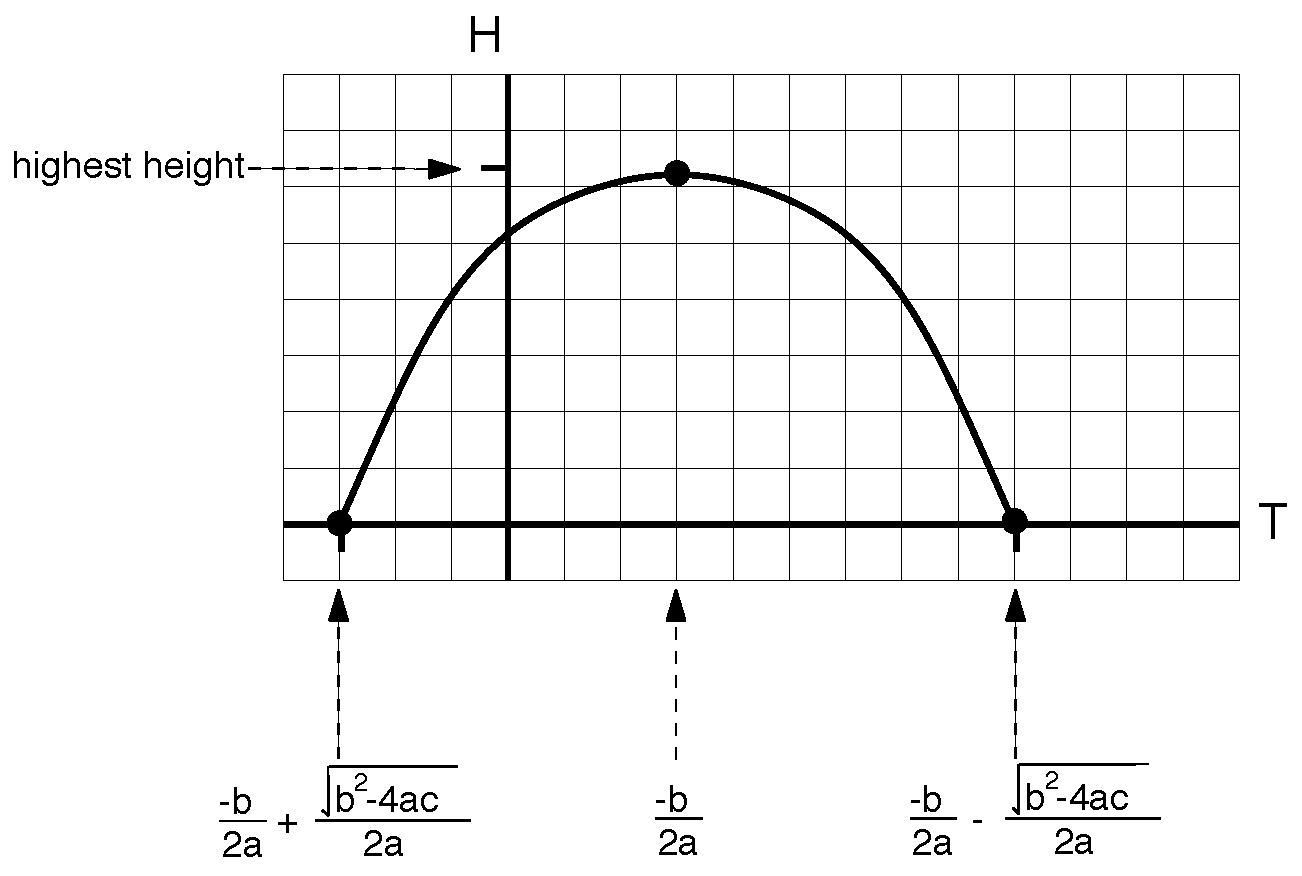
\includegraphics [width = 6in] {quadratic.pdf}}
\end{center}

Our graph was $\cap$ shaped parabola and so we found a maximum value.  The graph of a quadratic function might be $\cup$ shaped instead.  In that case evaluating at $T=\frac{-b}{2a}$ would give the minimum value. 

%
%\newpage

%%\section{Solving quadratic equations}

\begin{center}
\line(1,0){300} %\line(1,0){250}
\end{center}

\section*{Homework}

\noindent \textbf{Start by doing Practice exercises \#1-4 in the workbook.}

\bigskip

\noindent \textbf{Do you know \ldots}

\begin{itemize}
\item What a ``quadratic'' function is? 
\item How to solve a quadratic equation? 
\item When we use the \textsc{Quadratic Formula}?   \emph{Ask your instructor if you need to remember the \textsc{Quadratic Formula} or if it will be provided during the exam.}
\item How to solve a quadratic equation when the function is not set equal to zero? 
\item How to identify the values of $a, b, c$ in the formula? 
\item How to evaluate the formula (using your calculator)?   \item Why there are (usually) two solutions to a quadratic equation? 
\item How to decide which solution(s) from the \textsc{Quadratic Formula} are correct? 
\item What the graph of a quadratic function looks like? 
\item The value for the independent variable to find  the highest (or lowest) value of a quadratic function? 
 \item[~] \textbf{If you're not sure, work the rest of exercises and then return to these questions.  Or, ask your instructor or a classmate for help.}
\end{itemize}

\subsection*{Exercises}

\begin{enumerate} 
\setcounter{enumi}{4}

\item Claude is an excellent juggler.  Remember that the height $H$ feet of Claude's beanbag $T$ seconds after he throws it in the air is described by the equation $H = 3+15T-16T^2$. Answer each of the following question by the suggested method and then look back at the graph from earlier to make sure your answers make sense.
\begin{enumerate}
\item Use the \textsc{Quadratic Formula} to find when is the bean bag is 5 feet above ground?  Why do both answers make sense in the story?
\item When is the beanbag 8 feet above ground?  Try to use the \textsc{Quadratic Formula} to find the answer.  What happens?  Explain why it makes sense in the story that you can't solve this quadratic equation.
\item Claude decided that the beanbag was too high in the air, so he modified his throw slightly.  Now the height is given by $H = 3+14T-16T^2$.  What is the maximum height the beanbag will reach now?  \emph{Hint:  what number can you evaluate at?}
\end{enumerate}

\item The stopping distance for Jeff 's Cadillac Escalade is given by  $$D=.04S^2+1.47S$$ where $S$ is the speed of the car (in miles per hour) and $D$ is the stopping distance (in feet). Jeff took 183 feet to stop.  How fast was he going? 

\hfill \emph{Story also appears in Section 2.3}
\begin{enumerate}
\item Use successive approximation to estimate the answer to the nearest miles per hour.  Display your work in a table.
\item Show how to use the \textsc{Quadratic Formula} to solve the equation.
\end{enumerate}

\item A company produces backpacks.  The more they make, the less it costs for each one. The cost per backpack is given by the equation $$C = .01B^2 -1.2B + 50$$ where $C=$ cost per backpack (\$ per backpack) and $B=$ number of backpacks.

\hfill \emph{Story appears in 1.3 Exercises}
\begin{enumerate}
\item How many backpacks do they need to produce in order to hold costs to \$20/backpack?  Set up and solve a quadratic equation to find the answer.
\item Make a table of values and draw a graph of the function. Does your answer agree with your table and graph?  
\item What is the minimum price per backpack?  \emph{Hint:  evaluate at $T= \frac{-b}{2a}$.}
\end{enumerate}

\item Mrs.\ Weber's cooking class came up with the equation $$M = 1.2F^2+4F+7$$ to approximate the grilling time of a piece of fish depending on its thickness.  Here $M$ is the number of minutes to grill the fish and $F$ is the thickness of the fish in inches.  

\hfill \emph{Story appears in 1.1 and 2.3 Exercises}
\begin{enumerate}
\item If we want to make sure the fish will cook in under 20 minutes, what thickness steak can we have? Set up and solve a quadratic equation to find the answer.
\item Repeat for 10 minutes. 
\end{enumerate}

\item A company who makes electronics was doing great business in 1996, but sales quickly slid after 2000.  Their sales $M$ in millions of \$ $Y$ years from 1996 is given by the following equation $$M = 104.4+11.5Y-1.4Y^2$$
\hfill \emph{Story appears in 2.4 Exercises}
\begin{enumerate}
\item The company decided to declare bankruptcy when sales fell below \$20 billion.  In what year was that?    Show how to solve using the \textsc{Quadratic Formula.}
\item An analyst had suggested that they close down shop earlier, once sales were below \$50 billion.  In what year did sales fall that low? Show how to solve using the \textsc{Quadratic Formula.}
\item What year did sales \textbf{peak} (reach their highest value)?  
\end{enumerate} 

\item A kangaroo hops up in the air (and out) from a 10 foot cliff.  Her height above the ground, $K$ feet, after $T$ seconds is given by the equation $$K = 10 + 5.2T - 4.88T^2$$ 
\begin{enumerate}
\item Calculate the missing values in the table. 
\begin{center}
\begin{tabular} {|l|c|c|c|c|c|c|} \hline
T & 0 & .3 & .6 & .9 & 1.2 & 1.5 \\ \hline
K& 10 & 11.1208 & 11.3632  &  \hspace{.4in}    &  \hspace{.4in}   &6.82  \\ \hline
\end{tabular}
\end{center}
\item According to this equation, how high up in the air does the kangaroo get? 
Choose the appropriate value to plug into the equation.
\item When does the kangaroo land on the ground? 
Set up and solve an equation.
\item If she jumps up, but not out, when will she land on the cliff itself again, assuming the same equation holds?
\end{enumerate}

\end{enumerate}

